\documentclass[12pt]{article}
\usepackage{amsmath}
\usepackage{amssymb}
\usepackage{listings}
\usepackage{hyperref}
\usepackage{appendix}
\usepackage{graphicx}
\usepackage[margin=1in]{geometry}

\lstset{
language=C,
basicstyle=\small\sffamily,
numbers=left,
numberstyle=\tiny,
frame=tb,
columns=fullflexible,
showstringspaces=false
}

\title{\vspace{-1cm}Sparse Matrix Representation Using Finite State Transducers}
\author{\vspace{-1cm}Julian Knodt}

\setlength{\parindent}{0cm}
\setlength{\parskip}{\baselineskip}
\begin{document}

\maketitle
Professor Kai Li \\
COS 598D Systems \& ML

\begin{abstract}
Sparse Matrices are crucial for the efficient operation in many different contexts which lead to
dense operations such as in pruned neural nets or in sparse graph operations. Currently, there
exist many different formats for sparse matrices, differing in efficiency of matrix operations
and compression. Most popular among representations for unstructured sparse matrices are
Compressed Sparse Row(CSR), Coordinate Order(COO), and Compressed Sparse Column(CSC). We explore
an alternative unstructured sparse matrix format, based on a data structure commonly used in
string processing, finite state transducers. We find that the proposed structure can be within
an order of magnitude of efficiency on sparse matrix vector multiplication as compared to the
CSR format, and equivalent compression size, and with sparsity above 0.005, gets better
compression than CSR.
\end{abstract}

\section*{Introduction}
Dense matrices in general provide a continuous map of indices to values. Continuous, in this
case means that every index has a corresponding well-defined value. This is costly when the matrix has a
lot of redundancy, specifically if a lot of elements are $0$. Sparse matrix formats remove the assumption
of continuity in order to improve compression, and allow for faster iteration over non-zero
elements. The utilization of sparsity is harder to optimize for than it may appear as a lot of
performance gain for matrix operations is due to the easy parallelizability of elements for use
in CPU SIMD operations or on GPUs, both of which are readily available in a dense matrix
format. Yet, there are many applications from which sparse matrices naturally arise such as
neural nets or social connection graphs, and the cost of representing them as dense matrices
becomes increasingly costly. Sparse matrices thus become essential to feasibility and efficiency
of many applications.

\section*{Approach}

Sparse matrices's API is much closer to that of an ordered map, in that most operations
such as sparse vector-multiplication rely on efficient ordered iteration over the elements, and
random access of elements might become more costly. CSR offers an extremely efficient way to
perform iteration by representing rows implicitly as a series of pointers into column indices.
While this approach works well for 2 dimensional tensors, generalizing it requires
re-implementing it with another level of indirection, and it would not be immediately compatible
with lower dimensional tensors. A more general sparse tensor representation should be able to
generalize to higher dimensional tensors without reimplementation, ideally without loss of
efficiency.

Traditionally, an ordered map might be represented by a binary tree key-value store. but this
assumes keys and doesn't remove a ton of repetition. An alternate ordered map format is the
\textit{Finite State Transducer}(FST), used for efficient prefix and suffix compression when
storing a lot of strings. Consider indices into a matrix as strings, then it seems natural to
use finite state transducers as a way to encode sparse matrices. Notably, they present extremely
efficient compaction of large sets of strings, while having little overhead for having a diverse
set of strings with little overlap. Memory efficiency, while not directly correlated to speed,
tends to lend itself to fast iteration.

Some notable differences between a general finite state transducer and one used to encode a
matrix is that for a matrix every key's length is fixed and known ahead of time, thus we can
remove some of the dynamics elements in an FST such as checking whether a specific character is
the end of a string or not. In addition, we seek to optimize iteration efficiency, whereas most
FST's might look to optimize for flexibility of key search.

We look to match the efficacy of CSR matrix-vector multiplication and matrix-matrix
multiplication, but allow for easy representation of higher dimensional matrices.

\section*{Implementation}

We look at a CPU implementation of a finite state transducer with manual memory management for
maximal control over efficiency. We modify an existing FST
library\footnote{\url{https://github.com/BurntSushi/fst/tree/master}} and extend it to support
arbitrary element types, as well as multiple different length input encodings (byte, short,
int), and other modifications.

In order to have some comparison, we implement a simple CSR
format and compare to that. Notably, both the FST-backed and the CSR-backed versions do not have
BLAS optimizations\footnote{For a more efficient BLAS implementation, see
\href{https://software.intel.com/en-us/mkl-developer-reference-c-sparse-blas-csr-matrix-storage-format}
{Intel's implementation}.} We choose not to compare to a BLAS implementation, as it would take
significant engineering effort to implement something at the same level of efficiency. In general,
we expect the time complexity to be the same, but there to be a constant factor increase.
Therefore, the relative efficiency is an accurate measure of how an efficient variation of our
proposed idea would compare our implementation to an efficient CSR implementation.

Herein, we describe the major modifications made to the FST library, which primarily consist of
reduction of complexity, denoting contiguous ranges of elements, and creating multiple iteration
strategies.


\subsection*{Reducing Complexity in the FST Library}

Due to differing desires for a general purpose FST library and one designed for matrices,
different trade-offs must be made in the underlying design. Specifically, additional costs at
run-time might be alright if that leads to an improvement of the compression ratio. In our case,
that trade-off is inverted, where lower run-time at the cost of increased efficiency is an
acceptable trade-off. Due to that swapped expectation, we make some notable changes to the
underlying library.

% 1. Compile-time fixed sized input sequences
% 2. Reduced compilation variants
% 3. Generalized output types
% 4. Striated element sequences

\subsection*{Marking Contiguous Ranges}

% TODO discuss why marking ranges as continuous was useful for iteration speed

\subsection*{Iteration}

% Discuss iteration using an explicit marker, parallel iteration, etc

\section*{Experiments}

All experiments were run on a machine on a Ubuntu Linux Machine, with 1 \textit{x86\_64} Intel
i7-4770 CPU @ 3.4 GHz.

We looked at matrices from
\href{https://github.com/google-research/google-research/tree/master/state_of_sparsity}{Google's
sparse matrix research}, using absolute thresholdin

We find that for similar input sizes, the cost in number of bytes for CSR and our proposed
format are near equivalent. As demonstrated in Figure \ref{fig:sparsity}. While not showing any
significant gains over the CSR format, when looking at higher dimensional tensors we expect it
to maintain a similar level of efficiency for sparsity.

\begin{center}
\begin{figure}
  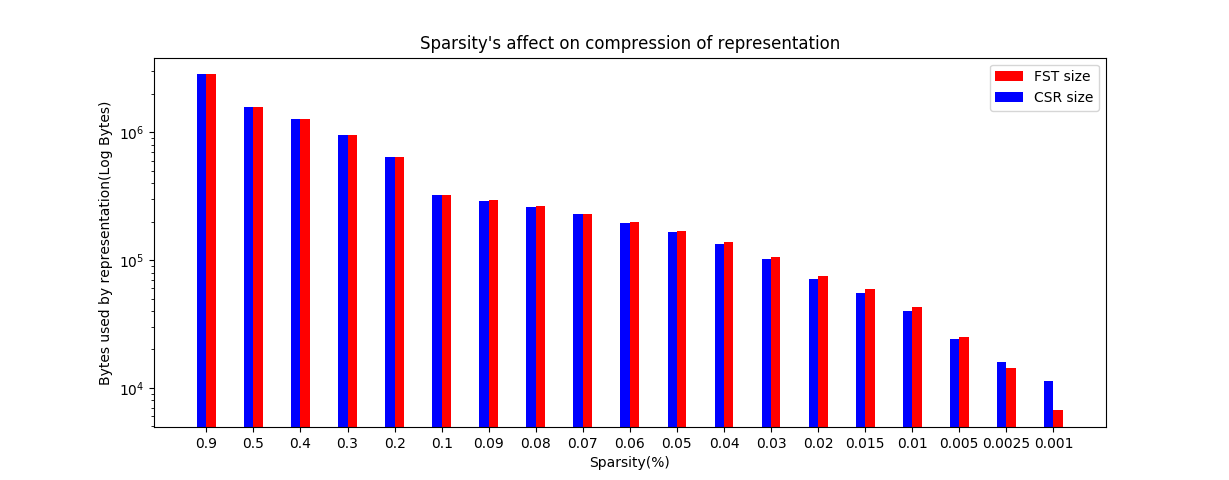
\includegraphics[width=\textwidth]{sparsity}
  \caption{The number of bytes used between a CSR format and the proposed FST format does not
differ. At extremely low sparsity, our format appears to be better, but since the overall
cost is quite small this benefit might not be significant.}
  \label{fig:sparsity}
\end{figure}
\end{center}



\section*{Results}

\appendix
\section{General Notes}
During work on this project, there were some notable realizations I came to about sparse matrix
structure.

Sparse matrices that I've looked at often do not distinguish between the indexing structure and
the elements themselves. Most of the work in sparse matrices is done on creating a structure
that specifies an efficient way to iterate through an array of elements. I have not seen a clear
distinction made between the efficiency of the indexing structure and how one can effectively
induce such a structure in a matrix. I think it might be productive to make such a distinction,
as I found it to be the case that blending iteration and indexing with the actual values in the
matrix lead to inefficiency, as one could insert the values in the matrix into the FST. In the
end, I switched to just maintaining a pointer into a contiguous array of elements and that lead
to a large performance gain because it meant in some cases I could mark elements as being ranges
over contiguous blocks, leading to efficient iteration.

\section{Convolution Algorithm with 2D Circular Buffer}
While working on this project, I realized that introducing a 2D circular buffer as an
intermediate buffer for partial sums reduces the
number of writes to the backing array. While this is not especially notable in the case of
convolving with one array, it might have some benefit when there are multiple writers, such as
when performing convolution over multiple channels in parallel to reduce memory thrashing.


\end{document}
